% Generated atomically by embed-optim-render-paper-results.
\begin{table*}[t]
\centering
\small
\begin{tabular}{llcc}
\toprule
Model & Optimizer & Final nDCG@10 & Rates reaching AdamW target \\
\midrule
DenseOn & AdamW & 0.5858 & 2/4 \\
DenseOn & Muon & 0.5901 & 3/4 \\
DenseOn & NorMuon & 0.5910 & 3/4 \\
\bottomrule
\end{tabular}
\caption{Discovery retrieval outcomes. Final scores are medians over four learning-rate points; target passage uses the frozen within-family AdamW reference.}
\label{tab:discovery-results}
\end{table*}

\begin{figure*}[t]
\centering
\begin{minipage}[t]{0.66\textwidth}
\centering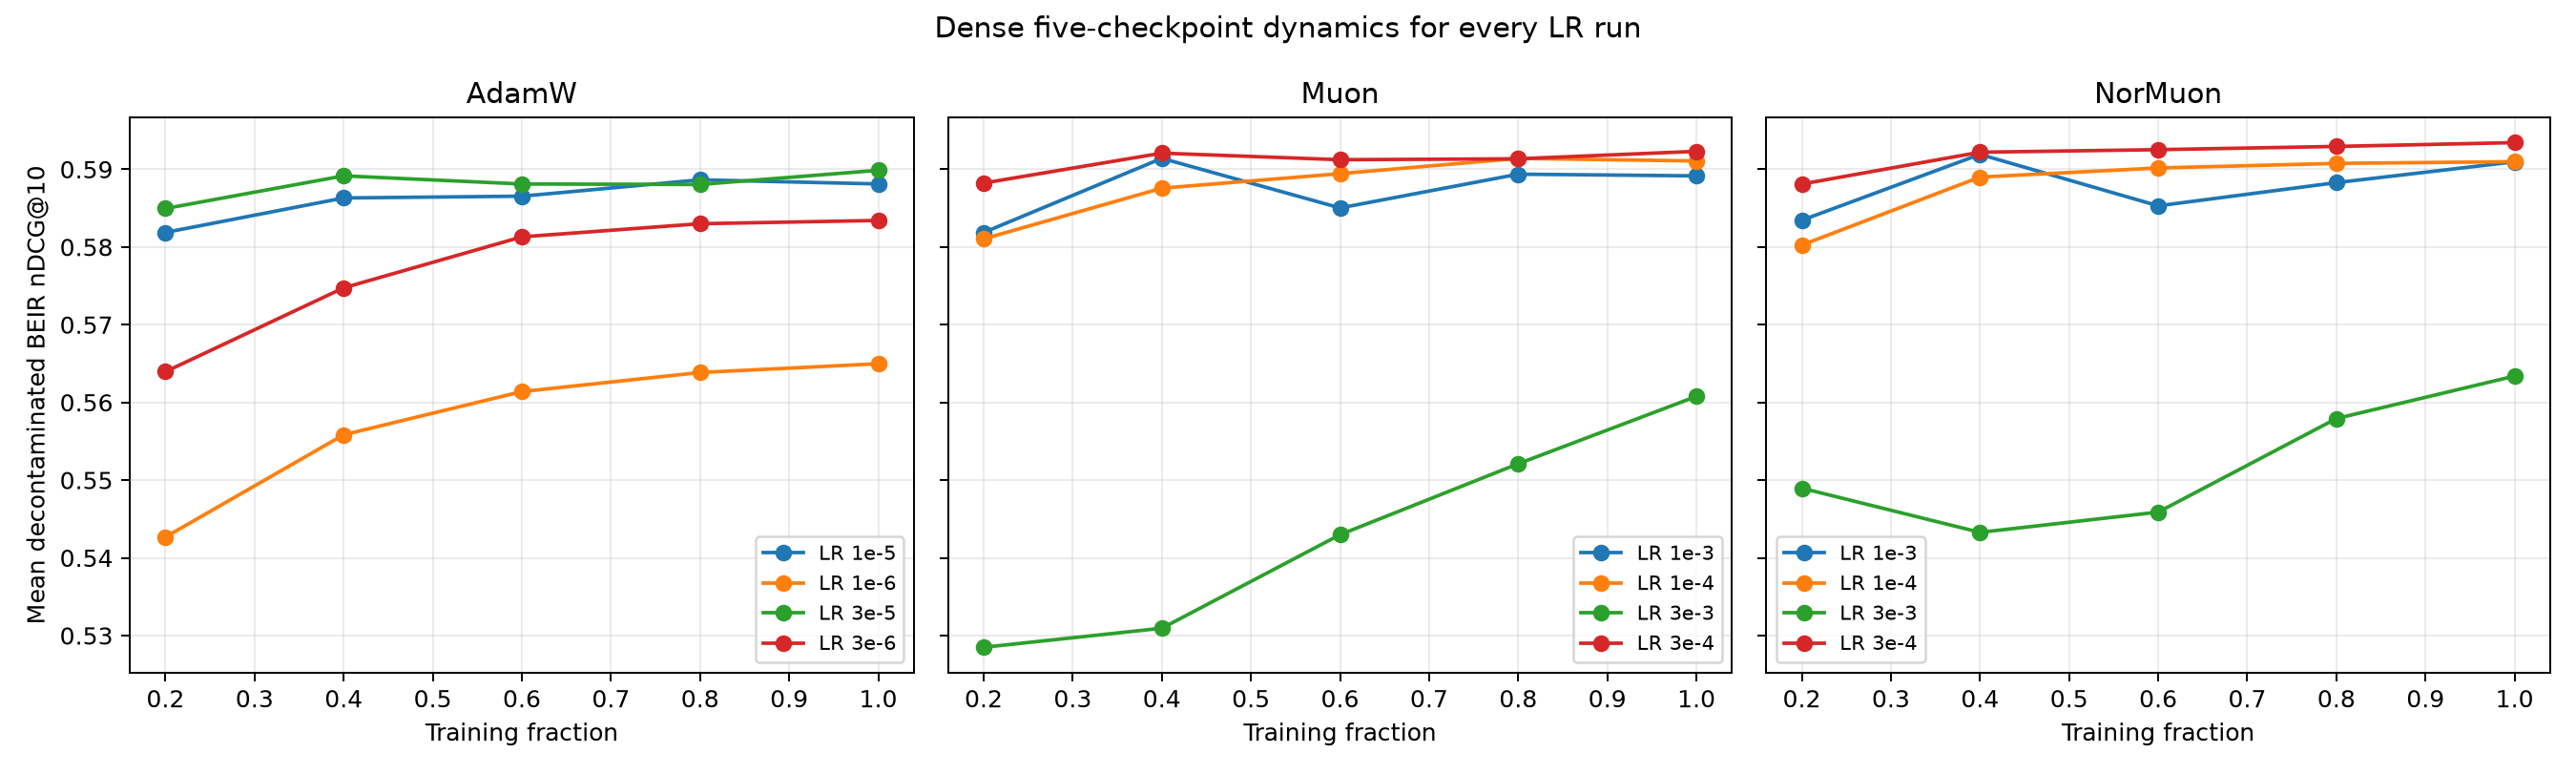
\includegraphics[width=\linewidth]{../reports/dense-discovery/figures/dense-training-dynamics-by-run.png}
\centering (a) Five-stage trajectories for every learning rate.
\end{minipage}\hfill
\begin{minipage}[t]{0.31\textwidth}
\centering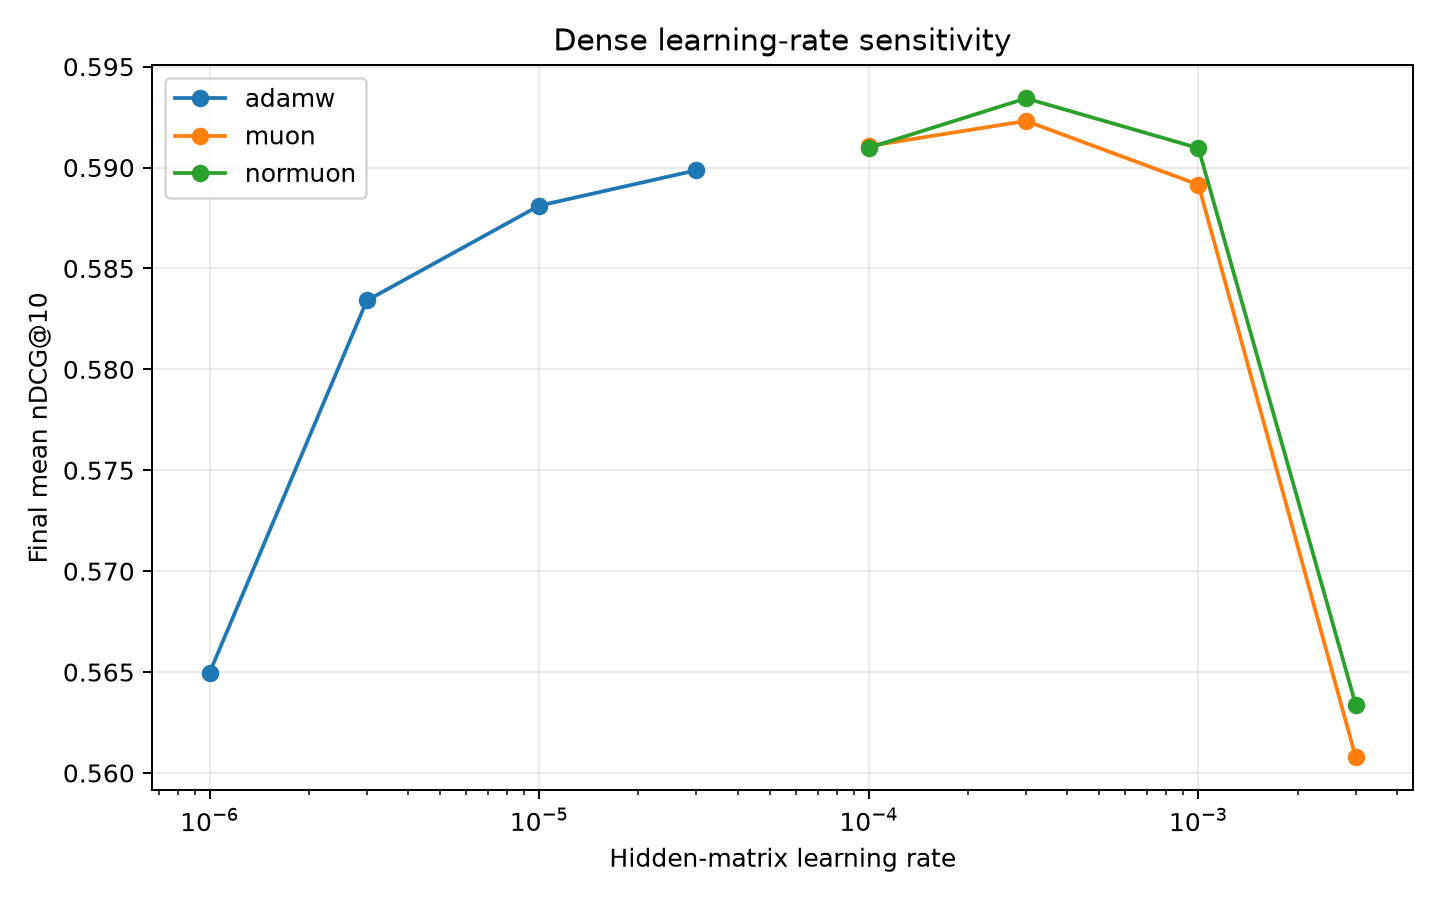
\includegraphics[width=\linewidth]{../reports/dense-discovery/figures/dense-lr-sensitivity.png}
\centering (b) Final-score learning-rate sensitivity.
\end{minipage}
\caption{DenseOn discovery dynamics. Panel (a) retains all 12 runs and all five checkpoints; panel (b) shows the final nDCG@10 response over each optimizer's frozen four-point learning-rate grid. These one-seed discovery curves are exploratory and do not replace the validation-frozen confirmation.}
\label{fig:dense-discovery-dynamics}
\end{figure*}
